\documentclass[10pt,x11names,table]{beamer}

\usetheme[progressbar=frametitle]{metropolis}
\usepackage{appendixnumberbeamer}
\usepackage{xcolor}

\usepackage{polyglossia}
\setmainlanguage{spanish}

\usepackage{listings}

\usepackage{booktabs}
\usepackage[scale=2]{ccicons}

\usepackage{pgfplots}
\usepgfplotslibrary{dateplot}

%ANIMACIONES
\usepackage{animate}
\usepackage{graphicx}
\usepackage[caption=false]{subfig}

\usepackage{xspace}

\newcommand*{\eg}{e.g.\@\xspace}
\newcommand*{\ie}{i.e.\@\xspace}

\let\oldquote\quote
\let\endoldquote\endquote
\renewenvironment{quote}[2][]
  {\if\relax\detokenize{#1}\relax
     \def\quoteauthor{#2}%
   \else
     \def\quoteauthor{#2~---~#1}%
   \fi
   \oldquote}
  {\par\nobreak\smallskip\hfill(\quoteauthor)%
   \endoldquote\addvspace{\bigskipamount}}
   
\usepackage{wrapfig}

\usepackage{subfig}
\usepackage{hyperref}
\usepackage{multicol}

\setbeamertemplate{bibliography item}[text]

\usepackage[font=small,skip=0pt, labelformat=empty]{caption}

\usepackage{dirtytalk}
\usepackage[acronym]{glossaries}
\makeglossaries

\newacronym{acgan}{ACGAN}{Auxiliary Classifier GAN}
\newacronym{ae}{AE}{Autoencoder}
\newacronym{ai}{AI}{Artificial Intelligence}
\newacronym{api}{API}{Application Programming Interface}
\newacronym{bert}{BERT}{Bidirectional Encoder Representations from Transformers}
\newacronym{brief}{BRIEF}{Binary Robust Independent Elementary Features}
\newacronym{brnn}{BRNN}{Bidirectional RNN}
\newacronym{bptt}{BPTT}{Backpropagation Through Time}
\newacronym{cbow}{CBOW}{Continous bag-of-words}
\newacronym{cnn}{CNN}{Convolutional Neural Network}
\newacronym{crnn}{CRNN}{Convolutional Recurrent Neural Network}
\newacronym{ddpm}{DDPM}{Denoising Diffusion Probabilistic Model}
\newacronym{ddim}{DDIM}{Denoising Diffusion Implicit Model}
\newacronym{diffit}{DiffiT}{Diffusion Vision Transformer}
\newacronym{dl}{DL}{Deep Learning}
\newacronym{dnn}{DNN}{Deep Neural Network}
\newacronym{dos}{DoS}{Denial of Service}
\newacronym{drnn}{DRNN}{Deep Recurrent Neural Network}
\newacronym{ecg}{ECG}{Electrocardiogram}
\newacronym{elmo}{ELMo}{Embedding from Language Model}
\newacronym{fast}{FAST}{Features from Accelerated Segment Test}
\newacronym{fid}{FID}{Fréchet Inception Distance}
\newacronym{foss}{FOSS}{Free and open-source software}
\newacronym{gan}{GAN}{Generative Adversarial Network}
\newacronym{glove}{GloVe}{Global Vectors for Word Representation}
\newacronym{gpu}{GPU}{Graphics Processing Unit}
\newacronym{gru}{GRU}{Gated Recurrent Unit}
\newacronym{ilsvrc}{ILSVRC}{ImageNet Large Scale Visual Recognition Challenge}
\newacronym{is}{IS}{Inception Score}
\newacronym{kid}{KID}{Kernel Inception Distance}
\newacronym{ldm}{LDM}{Latent Diffusion Model}
\newacronym{lstm}{LSTM}{Long Short-Term Memory}
\newacronym{mape}{MAPE}{Mean Absolute Perentage Error}
\newacronym{ml}{ML}{Machine Learning}
\newacronym{mlp}{MLP}{Multilayer Perceptron}
\newacronym{mmd}{MMD}{Maximum Mean Discrepancy}
\newacronym{mse}{MSE}{Mean Squared Error}
\newacronym{ner}{NER}{Named Entity Recognition}
\newacronym{nlg}{NLG}{Natural Language Generation}
\newacronym{nlp}{NLP}{Natural Language Processing}
\newacronym{nlu}{NLU}{Natural Language Understanding}
\newacronym{nn}{NN}{Neural Network}
\newacronym{ocr}{OCR}{Optical Character Recognition}
\newacronym{onnx}{ONNX}{Open Neural Network Exchange}
\newacronym{pmml}{PMML}{Predictive Model Markup Language}
\newacronym{relu}{ReLU}{Rectified Linear Unit}
\newacronym{rest}{REST}{Representational State Transfer}
\newacronym{rnn}{RNN}{Recurrent Neural Network}
\newacronym{sae}{SAE}{Stacked Autoencoder}
\newacronym{sift}{SIFT}{Scale-Invariant Feature Transform}
\newacronym{slam}{SLAM}{Simultaneous Localization and Mapping}
\newacronym{sru}{SRU}{Single Recurrent Unit}
\newacronym{surf}{SURF}{Speeded-Up Robust Features}
\newacronym{svm}{SVM}{Support Vector Machine}
\newacronym{vae}{VAE}{Variational Autoencoder}
\newacronym{vgg}{VGG}{Visual Geometry Group}
\newacronym{vit}{ViT}{Vision Transformer}
\newacronym{wsgi}{WSGI}{Web Server Gateway Interface}
\newacronym{xai}{XAI}{eXplainable Artificial Intelligence}
\newacronym{yolo}{YOLO}{You Only Look Once}
\newacronym{zsl}{ZSL}{Zero-shot Learning}
\subtitle{Métodos Generativos, curso 2024-2025}

\date{\today}
\author{Guillermo Iglesias, guillermo.iglesias@upm.es \newline
Jorge Dueñas Lerín, jorge.duenas.lerin@upm.es  \newline
Félix Fuentes Hurtado, felix.fuentes@upm.es}

\institute{Escuela Técnica Superior de Ingeniería de Sistemas Informáticos | UPM \newline
\hbox{} \newline \ccbysa \hspace{0.1pt} \ccNonCommercial}

%%%%%%%%%%%%%%%%%%%%%%%%%%%%%%%%%%%%%       
\title{Redes convolucionales}

\begin{document}
\maketitle

\section{Motivación}

\begin{frame}{Problemas del perceptrón}
Como anteriormente se ha visto, una arquitectura de \alert{perceptrón} es capaz de tratar con imágenes. Para ello las matrices \alert{bidimensionales} o \alert{tridimensionales} son transformadas a un vector \alert{unidimensional} con la operación de \say{\alert{flatten}}.

\begin{figure}
    \centering
    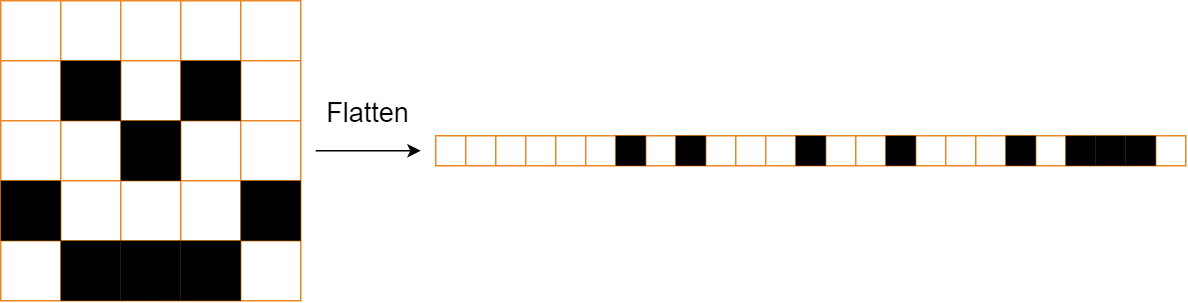
\includegraphics[width=\textwidth]{figures/Tema 3/Flatten.png}
\end{figure}
\end{frame}

\begin{frame}{Problemas del perceptrón}
El principal \alert{inconveniente} de esta aproximación es que se pierde toda la información \alert{espacial} de la imagen.

Esto hace que se pierdan las \alert{relaciones} de \alert{distancia} y \alert{color}.

Otro problema es la \alert{enorme} magnitud de las redes creadas de esta manera.

\centering
{\Large 512x512x3 píxeles = 786.432 neuronas entrada}
\end{frame}

\begin{frame}{Redes convolucionales}
Las redes neuronales \alert{convolucionales} surgen para adaptar las redes neuronales al \alert{tratamiento de imágenes}.

Los principales beneficios de su uso son los siguientes:
\begin{itemize}
    \item Aprovechamiento de la información \alert{espacial}.
    \item Reducción del número de \alert{parámetros}.
    \item \alert{Invarianza} aprendida de los datos.
\end{itemize}
\end{frame}

\section{Fundamentos de las redes convolucionales}

\begin{frame}{Operación de convolución}
La operación de \alert{convolución} consiste en la \alert{combinación lineal} de una ventana de píxeles de una imagen.

Para ello hay dos elementos fundamentales:
\begin{itemize}
    \item \alert{Imagen de entrada}: Una matriz \alert{bidimensional} de datos (normalmente normalizada a \alert{[-1, 1]} o \alert{[0, 1]}).
    \item \alert{Filtro o kernel}: Una matriz (normalmente de 3x3 o 5x5) con la que se realizará la \alert{combinación lineal} de los elementos de la imagen.
\end{itemize}

\begin{figure}
    \centering
    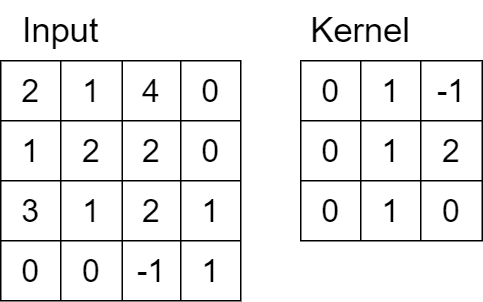
\includegraphics[width=0.5\textwidth]{figures/Tema 3/Convolucion2D_1.png}
\end{figure}
\end{frame}

\begin{frame}{Operación de convolución}
La salida se calcula  haciendo una \alert{combinación lineal} de cada región de la imagen. De esta manera la salida contiene la activación de cada zona de la imagen.

Esta región que el \alert{kernel} es capaz de \alert{observar} se conoce como \alert{campo receptivo}.

\begin{figure}
    \centering
    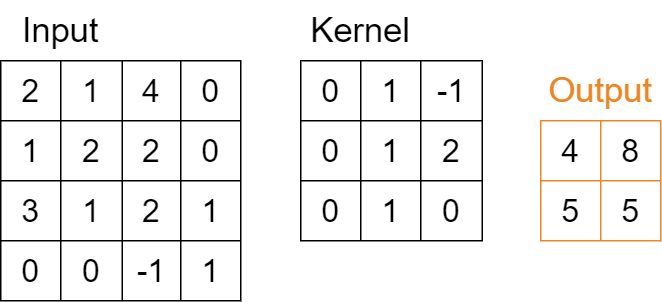
\includegraphics[width=0.7\textwidth]{figures/Tema 3/Convolucion2D_2.png}
\end{figure}
\end{frame}


\begin{frame}{Ejemplo de convolución 2-D}
\begin{figure}
    \centering
    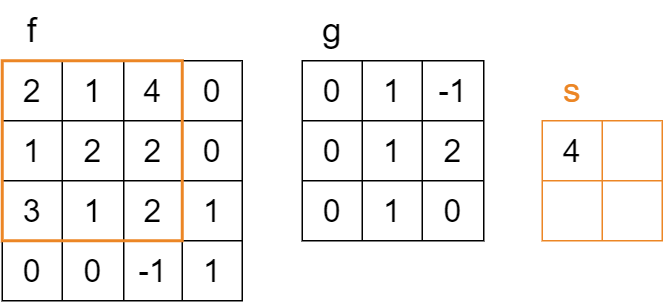
\includegraphics[width=0.8\textwidth]{figures/Tema 2/Convolucion2D_2.png}
\end{figure}
\end{frame}

\begin{frame}{Ejemplo de convolución 2-D}
\begin{figure}
    \centering
    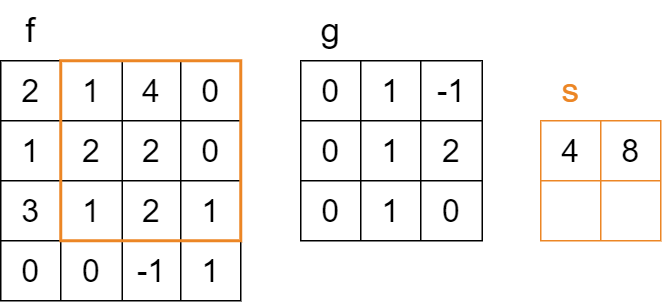
\includegraphics[width=0.8\textwidth]{figures/Tema 2/Convolucion2D_3.png}
\end{figure}
\end{frame}

\begin{frame}{Ejemplo de convolución 2-D}
\begin{figure}
    \centering
    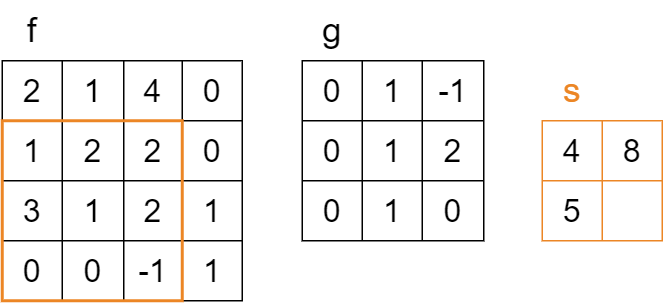
\includegraphics[width=0.8\textwidth]{figures/Tema 2/Convolucion2D_4.png}
\end{figure}
\end{frame}

\begin{frame}{Ejemplo de convolución 2-D}
\begin{figure}
    \centering
    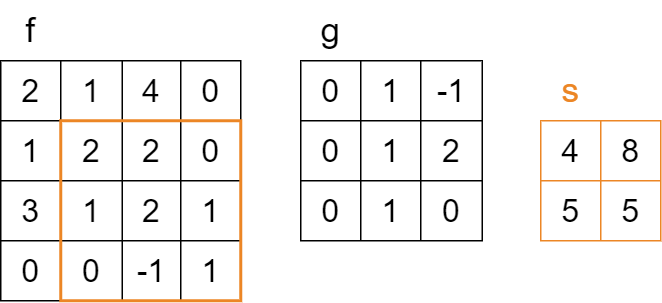
\includegraphics[width=0.8\textwidth]{figures/Tema 2/Convolucion2D_5.png}
\end{figure}
\end{frame}

\begin{frame}{Ejemplo de convolución 2-D}
\begin{figure}
    \centering
    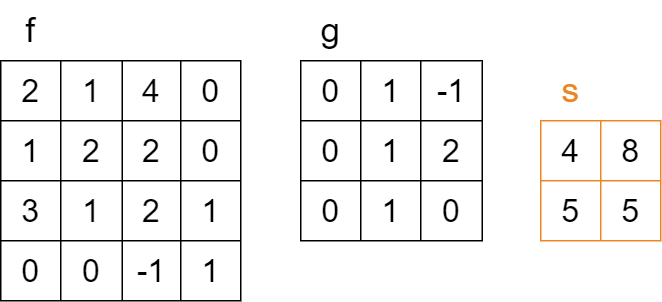
\includegraphics[width=0.8\textwidth]{figures/Tema 2/Convolucion2D_Res.png}
\end{figure}
\end{frame}

\begin{frame}{Campo receptivo}
La salida de la \alert{operación} tiene como objetivo la \alert{extracción de características} de las distintas \alert{regiones de la imagen}.

El \alert{campo receptivo} de cada celda de la salida se \alert{activa} cuando detecta una \alert{estructura de interés}.

\begin{figure}
    \centering
    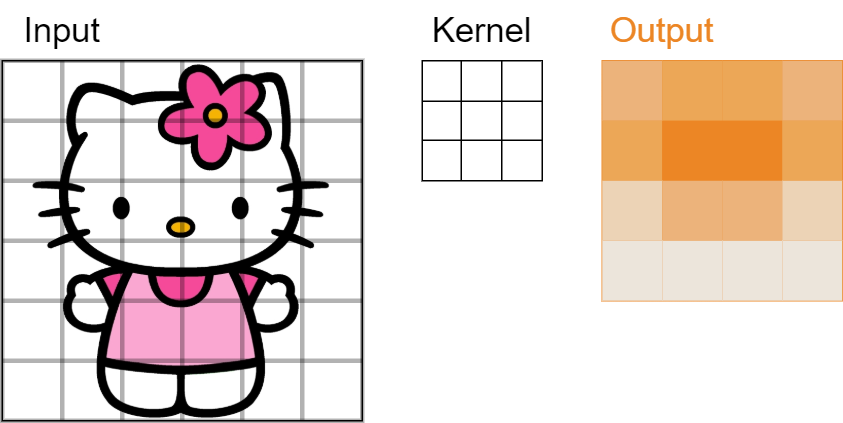
\includegraphics[width=\textwidth]{figures/Tema 3/ReceptiveActivation.png}
\end{figure}
\end{frame}

\begin{frame}{Campo receptivo}
La salida de la \alert{operación} tiene como objetivo la \alert{extracción de características} de las distintas \alert{regiones de la imagen}.

El \alert{campo receptivo} de cada celda de la salida se \alert{activa} cuando detecta una \alert{estructura de interés}.

\begin{figure}
    \centering
    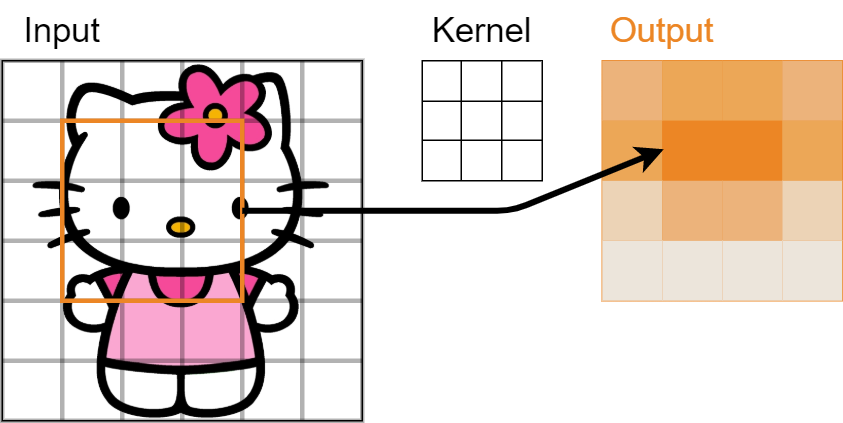
\includegraphics[width=\textwidth]{figures/Tema 3/ReceptiveActivation_1.png}
\end{figure}
\end{frame}

\begin{frame}{De neuronas a convoluciones}
Una \alert{red de neuronas} convolucional sustituye las capas \alert{densas} por capas \alert{convolucionales}.

Cada capa convolucional está compuesta por una \alert{serie} de \alert{filtros} de igual tamaño. Estos filtros se encargan de realizar el procesamiento de la información.

\begin{figure}
    \centering
    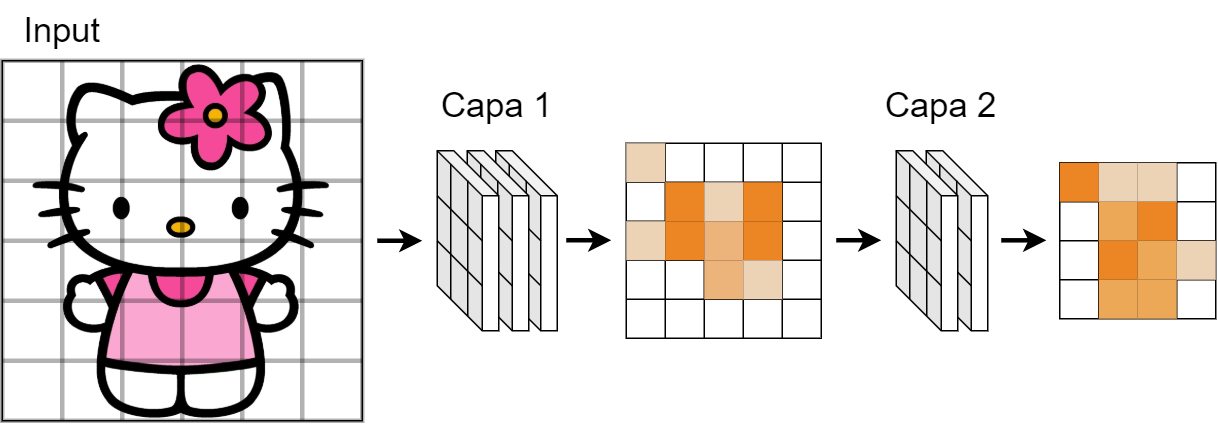
\includegraphics[width=\textwidth]{figures/Tema 3/CNN_Net.png}
\end{figure}
\end{frame}

\begin{frame}{De neuronas a convoluciones}
Cada \alert{filtro} de la red está compuesto por una serie de \alert{neuronas}. Estas, igual que con las redes \alert{tradicionales} tienen un \alert{peso} asociado. Este peso es el que regula cómo se realiza la \alert{convolución}.

\begin{figure}
    \centering
    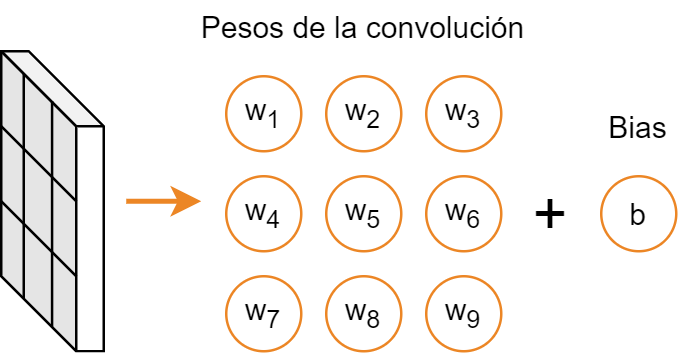
\includegraphics[width=\textwidth]{figures/Tema 3/ConvNeuron.png}
\end{figure}
\end{frame}

\begin{frame}{De neuronas a convoluciones}
Tras haber realizado la \alert{convolución} de unos datos de entrada, el resultado pasa por una \alert{activación} a través de una \alert{función no lineal}, tal y como sucede en las redes neuronales densas.

\begin{figure}
    \centering
    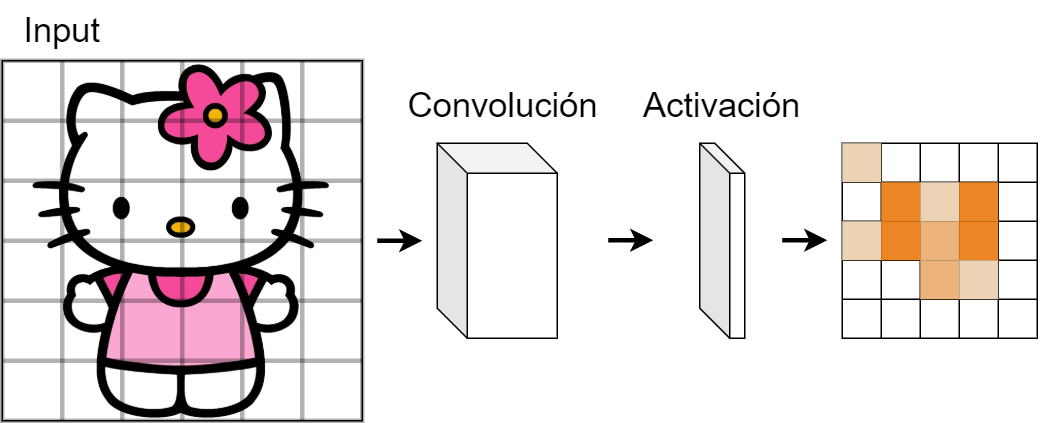
\includegraphics[width=\textwidth]{figures/Tema 3/ConvActivation.png}
\end{figure}
\end{frame}

\begin{frame}{Padding en la convolución}
Para controlar las \alert{dimensiones de salida} de cada capa convolucional se aplica un \textit{\alert{padding}} a la imagen de entrada. Este consiste en un marco de \say{\alert{0}} que evita la reducción dimensional.

\begin{figure}
    \centering
    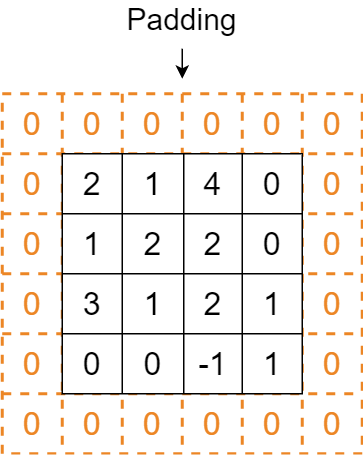
\includegraphics[width=0.4\textwidth]{figures/Tema 2/Padding.png}
\end{figure}
\end{frame}

\begin{frame}{Padding en la convolución}
Existen dos \alert{configuraciones} predominantes para la elección de padding en la librería \alert{keras}:
\begin{itemize}
    \item \textbf{\alert{Valid}}: No se aplica \alert{ningún} padding.
    \item \textbf{\alert{Same}}: Se aplica un padding que haga que la \alert{dimensión de salida} sea igual a la de \alert{entrada}.
    
    \vfill
    {\large \textbf{Ejemplo}: Para una imagen de 16x16 píxeles y un filtro de 3x3, el padding \say{same} sería de 1 píxel.}
\end{itemize}
\end{frame}

\begin{frame}{Resultado de una capa convolucional}
Cada \alert{capa convolucional} está formada por una serie de convoluciones. Las \alert{dimensiones de salida} de cada capa vienen dadas por:
\begin{itemize}
    \item \alert{Alto y ancho}: Dependen de las dimensiones de los \alert{datos recibidos}, el tamaño de \alert{kernel} y el \alert{padding} utilizado.
    \item \alert{Profundidad}: Corresponde con el \alert{número de filtros} aplicados a los datos.
\end{itemize}
\end{frame}

\begin{frame}{Resultado de una capa convolucional}
\begin{figure}
    \centering
    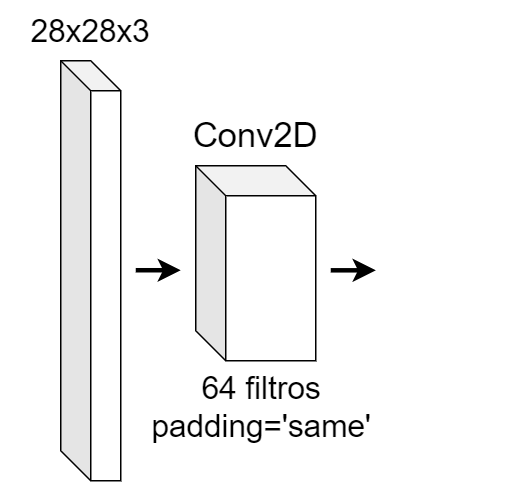
\includegraphics[width=0.7\textwidth]{figures/Tema 3/ConvDimensions_1.png}
\end{figure}
\end{frame}

\begin{frame}{Resultado de una capa convolucional}
\begin{figure}
    \centering
    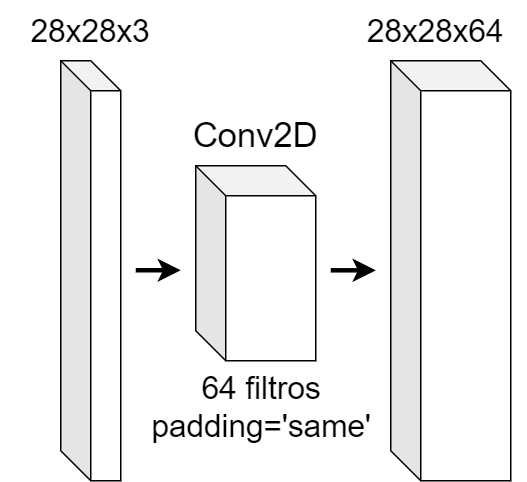
\includegraphics[width=0.7\textwidth]{figures/Tema 3/ConvDimensions_2.png}
\end{figure}
\end{frame}

\begin{frame}{Resultado de una capa convolucional}
\begin{figure}
    \centering
    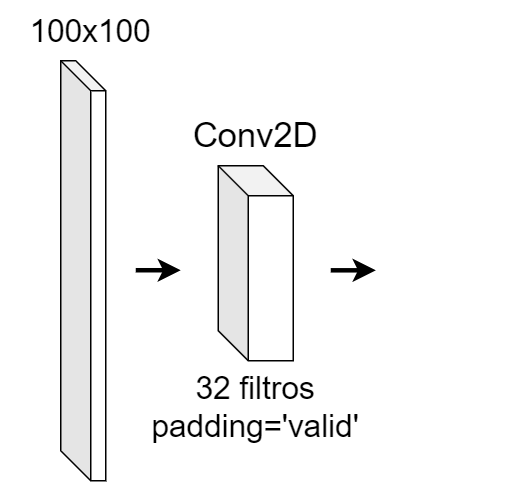
\includegraphics[width=0.7\textwidth]{figures/Tema 3/ConvDimensions_3.png}
\end{figure}
\end{frame}

\begin{frame}{Resultado de una capa convolucional}
\begin{figure}
    \centering
    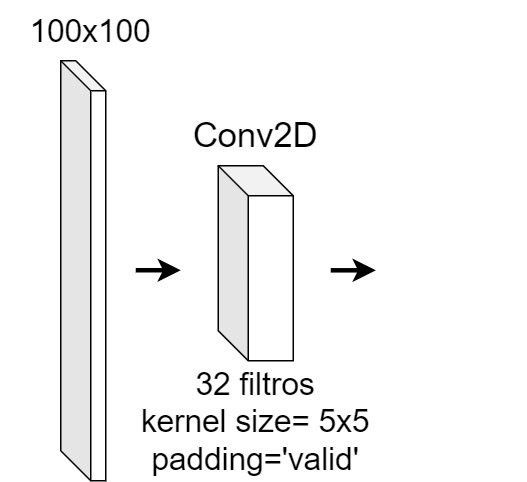
\includegraphics[width=0.7\textwidth]{figures/Tema 3/ConvDimensions_4.png}
\end{figure}
\end{frame}

\begin{frame}{Resultado de una capa convolucional}
\begin{figure}
    \centering
    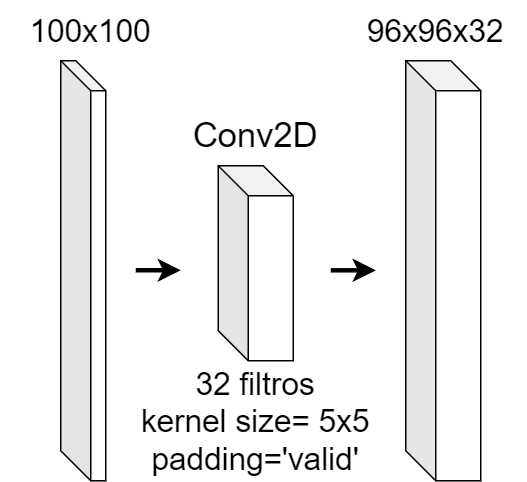
\includegraphics[width=0.7\textwidth]{figures/Tema 3/ConvDimensions_5.png}
\end{figure}
\end{frame}

\begin{frame}{Strides en la convolución}
Los \alert{\textit{strides}} o pasos de una convolución corresponden con el número de casillas que se desplaza \alert{horizontal} y \alert{verticalmente} el filtro al realizar la convolución.

\begin{figure}
    \centering
    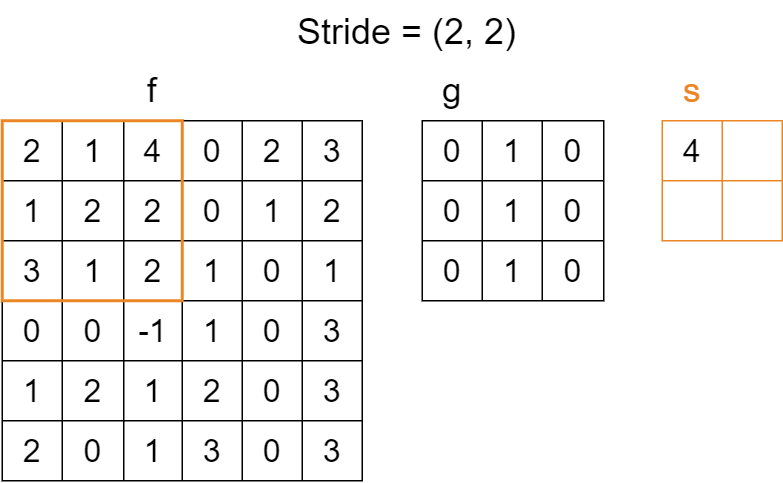
\includegraphics[width=0.9\textwidth]{figures/Tema 2/Strides2x2_2.png}
\end{figure}
\end{frame}

\begin{frame}{Strides en la convolución}
Los \alert{\textit{strides}} o pasos de una convolución corresponden con el número de casillas que se desplaza \alert{horizontal} y \alert{verticalmente} el filtro al realizar la convolución.

\begin{figure}
    \centering
    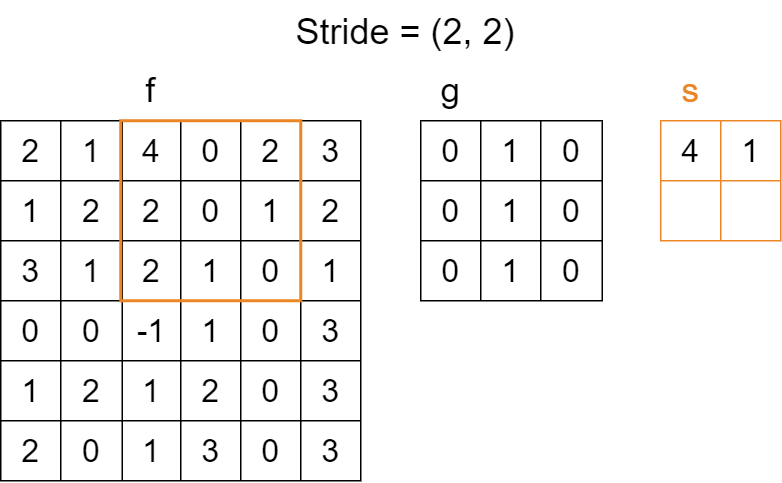
\includegraphics[width=0.9\textwidth]{figures/Tema 2/Strides2x2_3.png}
\end{figure}
\end{frame}

\begin{frame}{Strides en la convolución}
Los \alert{\textit{strides}} o pasos de una convolución corresponden con el número de casillas que se desplaza \alert{horizontal} y \alert{verticalmente} el filtro al realizar la convolución.

\begin{figure}
    \centering
    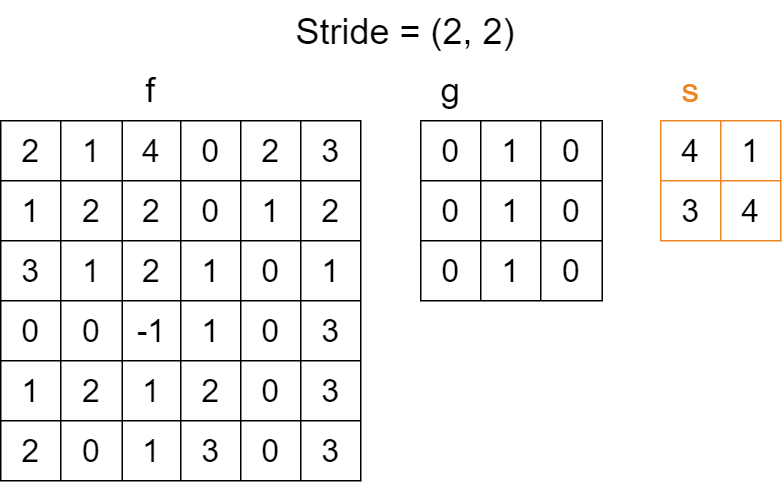
\includegraphics[width=0.9\textwidth]{figures/Tema 2/Strides2x2_Res.png}
\end{figure}
\end{frame}

\begin{frame}{Hiperparámetros de una convolución 2D}
La capa \alert{Conv2D} de la libería \alert{keras} tiene una serie de \alert{hiperparámetros} que permiten su \alert{configuración}, dentro de los más importantes se encuentran:
\begin{itemize}
    \item \alert{filters}
    \item \alert{kernel\_size}
    \item \alert{strides}
    \item \alert{padding}
    \item \alert{activation}
\end{itemize}
\end{frame}

\begin{frame}{Hiperparámetros de una convolución 2D}
\begin{itemize}
    \item \alert{\Large filters}
\end{itemize}

Corresponden al \alert{número de filtros} que se le aplican a los datos de entrada.

\textit{Se define con un \alert{integer}.}

\begin{itemize}
    \item \alert{\Large kernel\_size}
\end{itemize}

Determina el \alert{tamaño de los filtros} que constituyen la capa.

\textit{Se define con un \alert{integer} para filtros \alert{cuadrados}, pero admite definir las dimensiones por separado en un vector \alert{(alto, ancho)}.}
\end{frame}

\begin{frame}{Hiperparámetros de una convolución 2D}
\begin{itemize}
    \item \alert{\Large strides}
\end{itemize}

Define el \alert{paso} de la convolución a lo largo de los ejes.

\textit{Se define con un \alert{integer} para un paso igual en \alert{ambos ejes}, pero admite definir cada dimensión por separado en un vector \alert{(alto, ancho)}.}

\begin{itemize}
    \item \alert{\Large padding}
\end{itemize}

Determina el \alert{padding} aplicado a los datos de entrada.

\textit{Se pueden definir las opciones \say{\alert{valid}} y \say{\alert{same}}.}
\end{frame}

\begin{frame}{Hiperparámetros de una convolución 2D}
\begin{itemize}
    \item \alert{\Large activation}
\end{itemize}

Define la \alert{activación} aplicada tras la convolución.

\textit{Dentro de las posibles activaciones se encuentran: relu, sigmoid, softmax, softplus, softsign, tanh, selu, elu, exponential.}

Existe la posibilidad de aplicar \alert{otras} activaciones así como activaciones \alert{custom}. Por ejemplo para aplicar la función \alert{LeakyReLU}.

\end{frame}

\begin{frame}{Parámetros de una convolución}
El número de parámetros de cada \alert{capa convolucional} viene dado por el tamaño del \alert{filtros}, el número de \alert{filtros} y la \alert{profundidad} de la información de la capa anterior:

\begin{equation}
    {\large ((kernel_{height} * kernel_{width} * depth_{input}) + 1) * filters}
\end{equation}

\begin{figure}
    \centering
    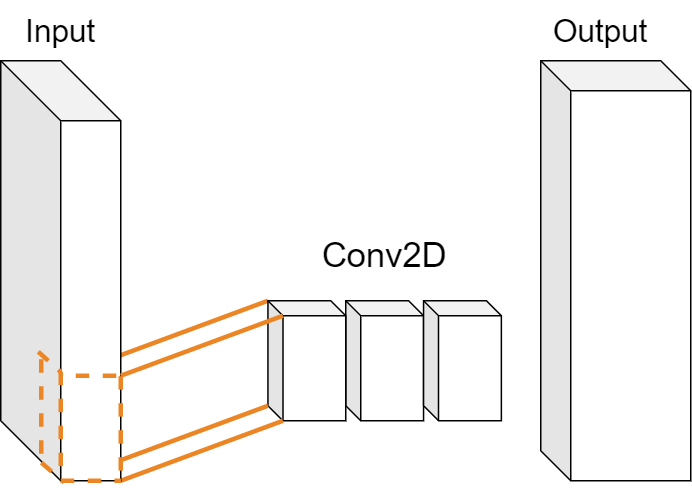
\includegraphics[width=0.6\textwidth]{figures/Tema 3/ConvParams.png}
\end{figure}
\end{frame}

\begin{frame}{Notebook de ejemplo, dimensiones de convolución}
El siguiente notebook contiene un breve código para explorar las \alert{dimensiones de salida} de una capa convolucional.

\begin{figure}
    \centering
    
\includegraphics[width=0.4\textwidth]{figures/GoogleColab.png}
\end{figure}
\begin{itemize}
    \centering
    \item {\Large \href{https://colab.research.google.com/drive/1UpvEAbh6kwSScuOJjf7228ZA5lWCHihO?usp=sharing}{1.2\_1-DimensionesConv2D.ipynb}}
\end{itemize}
\end{frame}

\begin{frame}{Web interactiva}
Web interactiva con resumen: \href{https://poloclub.github.io/cnn-explainer/}{https://poloclub.github.io/cnn-explainer/}
\end{frame}

\begin{frame}{Aprendizaje de una red convolucional}
A lo largo del tema se estudiarán distintas \alert{arquitecturas} construidas con capas convolucionales, pero cabe destacar que la \alert{estructura por capas} de estas redes consigue \alert{imitar} el procesamiento del \alert{cortex cerebral} del cerebro.

Las capas \alert{ocultas} de las redes convolucionales contienen una \alert{jerarquía} especializada en la tarea para la que se entrena.

Esto se traduce en que, la \alert{primeras} capas de la red se encargan de procesar información de \alert{bajo nivel}, como \alert{líneas} o \alert{curvas}; mientras que las \alert{últimas} capas se encargan de información de \alert{alto nivel}, como una cara o la silueta de un animal.
\end{frame}

\begin{frame}{Aprendizaje de una red convolucional}
\begin{figure}
    \centering
    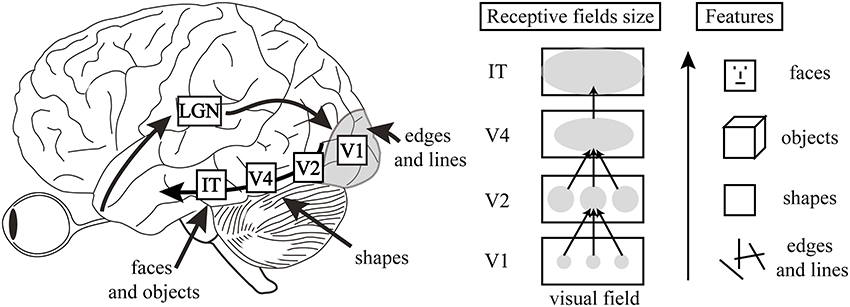
\includegraphics[width=\textwidth]{figures/Tema 3/Cortex.jpg}
    \caption{\cite{Cortex}}
\end{figure}
\end{frame}

\begin{frame}{Aprendizaje de una red convolucional}
\begin{figure}
    \centering
    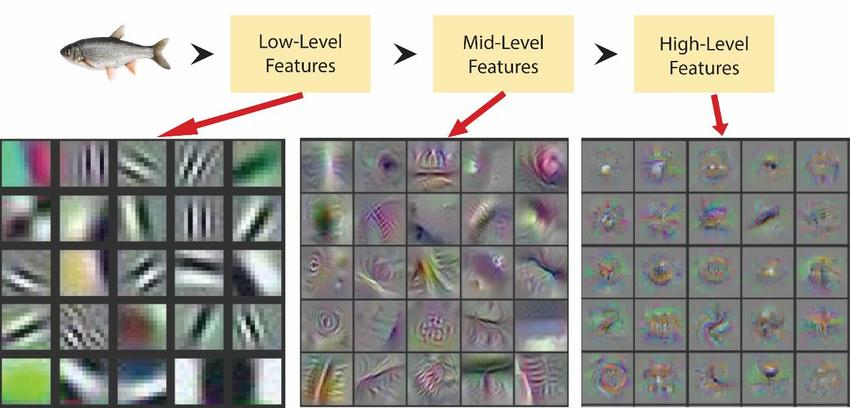
\includegraphics[width=\textwidth]{figures/Tema 3/ConvHierarchy.png}
    \caption{\cite{siddiqui2018automatic}}
\end{figure}
\end{frame}

\begin{frame}{Notebook de ejemplo, clasificador con redes convolucionales}
El siguiente notebook contiene un ejemplo de clasificador redes convolucionales.

\begin{figure}
    \centering
    
\includegraphics[width=0.4\textwidth]{figures/GoogleColab.png}
\end{figure}
\begin{itemize}
    \centering
    \item {\Large \href{https://colab.research.google.com/drive/19TfnBBgbAEDG4YC7EGwcJ6ETZi-xfAiL?usp=sharing}{1.2\_2-CNNImagenes.ipynb}}
\end{itemize}
\end{frame}

\addcontentsline{toc}{section}{Referencias}

\begin{frame}[allowframebreaks]{Referencias}
    \bibliographystyle{unsrt}
    \bibliography{references.bib}
\end{frame}

\end{document}